\documentclass[aspectratio=169]{beamer}

\usetheme{Madrid}
\usecolortheme{default}
\setbeamertemplate{navigation symbols}{}
\setbeamertemplate{footline}[frame number]

\usepackage[utf8]{inputenc}
\usepackage[T1]{fontenc}
\usepackage[brazil]{babel}
\usepackage{graphicx}
\usepackage{booktabs}
\usepackage{amsmath}

\title[Divisao e Conquista em Cryo-EM]{Reescrita e Implementacao de um Algoritmo de Divisao e Conquista para Segmentacao em Microscopia Eletronica}
\author{Vinicius Wanderley Arruda}
\institute{Projeto e Analise de Algoritmos \\ Prof. Warley Gramacho}
\date{09 de junho de 2026}

\begin{document}

\begin{frame}
  \titlepage
\end{frame}

\begin{frame}{Artigo Escolhido}
  \textbf{A Divide and Conquer Algorithm for Electron Microscopy Segmentation}

  \vspace{0.4cm}
  \begin{itemize}
    \item Autores: Ruba Jebril, Yingde Zhu, Wei Chen e Kamal Al Nasr.
    \item Publicado no ACM-BCB 2020.
    \item DOI: 10.1145/3388440.3414700.
    \item Tema: segmentacao de mapas de cryo-EM usando watershed e divisao e conquista.
  \end{itemize}
\end{frame}

\begin{frame}{Problema}
  \begin{itemize}
    \item A cryo-EM gera mapas tridimensionais de densidade de moleculas biologicas.
    \item Para modelar uma molecula, e necessario separar regioes associadas a cadeias ou subunidades.
    \item A segmentacao manual e demorada e depende de conhecimento especializado.
    \item O artigo busca acelerar a segmentacao usando divisao e conquista.
  \end{itemize}
\end{frame}

\begin{frame}{Conceitos Principais}
  \begin{block}{Cryo-EM}
    Tecnica experimental que permite observar moleculas biologicas congeladas em estado proximo ao natural.
  \end{block}

  \begin{block}{Mapa de densidade e voxel}
    O mapa de densidade e uma imagem 3D; cada pequena unidade de volume e chamada de voxel.
  \end{block}

  \begin{block}{Watershed}
    Tecnica de segmentacao baseada na ideia de separar regioes como bacias em uma superficie.
  \end{block}
\end{frame}

\begin{frame}{Ideia Geral do Algoritmo}
  \begin{enumerate}
    \item Gerar regioes preliminares com uma abordagem baseada em watershed.
    \item Dividir o mapa de densidade em subimagens menores.
    \item Resolver cada subimagem recursivamente.
    \item Combinar as regioes parciais ate chegar a no maximo $K$ regioes.
  \end{enumerate}

  \vspace{0.35cm}
  \centering
  \textbf{Dividir} $\rightarrow$ \textbf{Resolver subproblemas} $\rightarrow$ \textbf{Combinar}
\end{frame}

\begin{frame}{Segmentacao Preliminar}
  \begin{itemize}
    \item Filtra voxels abaixo de um limiar de densidade.
    \item Processa os voxels restantes em ordem decrescente de densidade.
    \item Cria regioes iniciais quando nao ha vizinhos ja segmentados.
    \item Associa voxels a regioes vizinhas quando ha contato local.
    \item Mescla regioes com base nos maximos locais.
  \end{itemize}
\end{frame}

\begin{frame}{Divisao}
  \begin{itemize}
    \item O artigo nao usa apenas divisao binaria.
    \item A proposta divide o mapa em aproximadamente $\sqrt{n}$ subimagens.
    \item Cada subimagem possui aproximadamente $\sqrt{n}$ voxels.
    \item Objetivo: reduzir o custo da fase de combinacao.
  \end{itemize}

  \vspace{0.3cm}
  \[
    D \rightarrow D_1, D_2, \ldots, D_{\sqrt{n}}
  \]
\end{frame}

\begin{frame}{Subproblemas}
  \begin{itemize}
    \item Cada subimagem e tratada como uma instancia menor do mesmo problema.
    \item O algoritmo chama a segmentacao recursivamente.
    \item Quando o bloco e pequeno, aplica-se a segmentacao preliminar.
    \item Essa etapa reduz o tamanho das combinacoes locais.
  \end{itemize}
\end{frame}

\begin{frame}{Combinacao}
  \begin{itemize}
    \item Cada subproblema pode gerar ate $K$ regioes.
    \item As regioes parciais sao reunidas.
    \item A fase de merge e aplicada novamente para chegar a no maximo $K$ regioes finais.
    \item O artigo tambem discute cuidado com fronteiras entre subimagens.
  \end{itemize}
\end{frame}

\begin{frame}{Analise de Complexidade}
  \begin{block}{Segmentacao preliminar}
    \[
      O(n \log n + m^2 \log m)
    \]
  \end{block}

  \begin{block}{Versao com divisao e conquista}
    \[
      T(n) = \sqrt{n}T(\sqrt{n}) + c(K\sqrt{n})^2\log(Kn)
    \]
    \[
      O(K^2 n \log n) \approx O(n \log n)
    \]
  \end{block}
\end{frame}

\begin{frame}{Implementacao Desenvolvida}
  \begin{itemize}
    \item Linguagem: Python.
    \item Entrada: matriz 2D sintetica de densidade.
    \item Saida: imagem com mapa de densidade e regioes segmentadas.
    \item A implementacao preserva a logica de divisao, recursao e merge.
    \item Repositorio: \texttt{github.com/ViiniDev/Atividade-de-PAA}
  \end{itemize}
\end{frame}

\begin{frame}{Demonstracao Pratica}
  \centering
  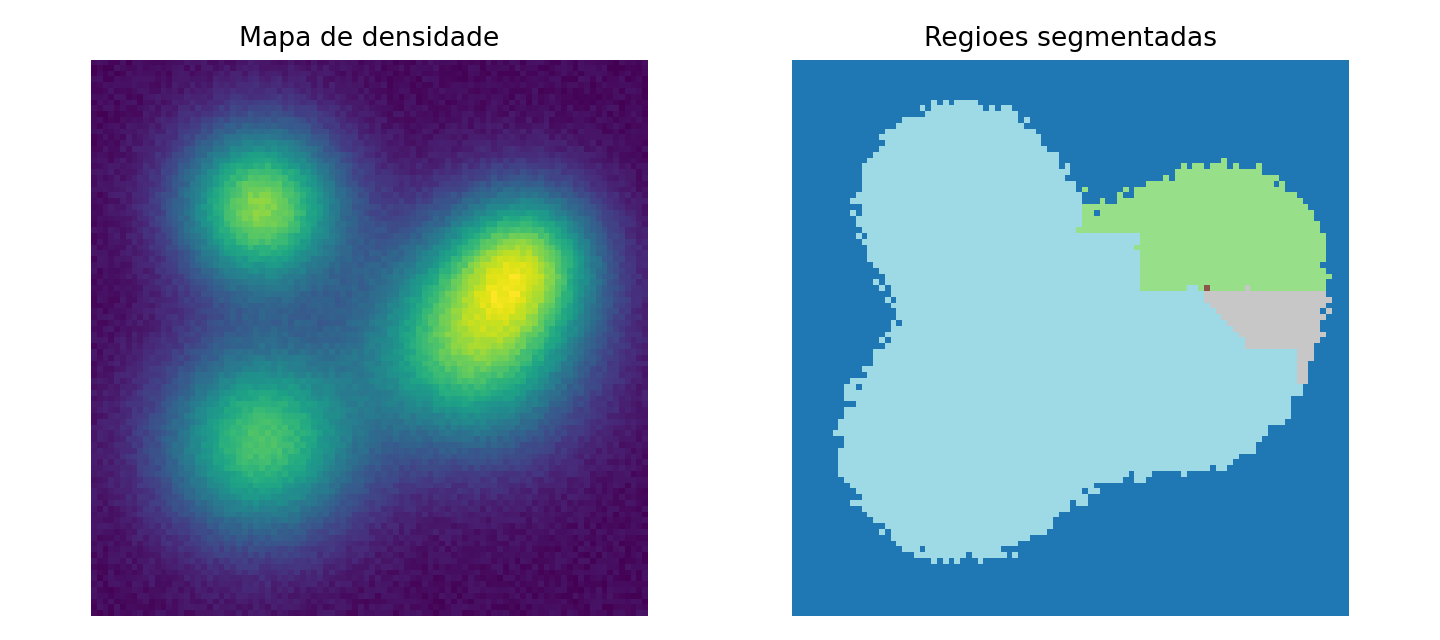
\includegraphics[width=0.88\textwidth]{demo_segmentacao.png}

  \vspace{0.2cm}
  \small Exemplo gerado pelo script \texttt{segmentacao\_dc.py}.
\end{frame}

\begin{frame}{Comparacao}
  \begin{table}
    \centering
    \small
    \begin{tabular}{p{0.25\textwidth}p{0.55\textwidth}}
      \toprule
      \textbf{Versao} & \textbf{Caracteristica} \\
      \midrule
      Preliminar & Watershed e merge sobre todas as regioes. \\
      Artigo & Divide o mapa, resolve subproblemas e combina regioes. \\
      Implementacao & Demonstra a tecnica em matriz 2D sintetica. \\
      \bottomrule
    \end{tabular}
  \end{table}

  \vspace{0.2cm}
  \small O artigo compara o metodo com o Segger e relata desempenho competitivo.
\end{frame}

\begin{frame}{Limitacoes}
  \begin{itemize}
    \item O artigo trabalha com mapas 3D reais de cryo-EM.
    \item A implementacao usa matriz 2D sintetica para facilitar demonstracao.
    \item A otimizacao de fronteiras foi representada de forma simplificada.
    \item A implementacao e didatica, nao uma ferramenta biologica completa.
  \end{itemize}
\end{frame}

\begin{frame}{Conclusao}
  \begin{itemize}
    \item O artigo aplica divisao e conquista a um problema real de segmentacao.
    \item A divisao reduz o custo de combinar muitas regioes preliminares.
    \item A implementacao demonstrou as etapas principais do algoritmo.
    \item O trabalho conecta a tecnica teorica com uma aplicacao pratica.
  \end{itemize}
\end{frame}

\begin{frame}{Perguntas}
  \centering
  \Large Obrigado!
\end{frame}

\end{document}
